\subsection{OSI参照モデル}

インターネットで利用されるプロトコルは、The Internet Engineering Task Force (IETF)という標準化
団体により策定され、その標準はRequest for Comments (RFC)という名のオープンな仕様として発行されている。
例えば、我々が利用しているインターネットプロトコルである
インターネットプロトコル バージョン4は、1981年に791番目のRFCとして策定された~\cite{RFC0791}。

IETF以外の通信に関する標準化団体としては
International Telecommunication Union Telecommunication Standardization Sector (ITU-T)や、
International Organization for Standardization (ISO)が存在する。
実は、1977年から1982年かけて、ITU-TやISOがコンピュータネットワークの標準通信プロトコルとして、
Open Systems Interconnection (OSI)の策定を行っていた。
その当時は標準的な通信プロトコルは存在せず、ベンダーごとに様々なプロトコルが利用されていたため、
通信プロトコルの統一化が求められていたのである。
しかしながら、最終的にOSIは主流とはならず、IETFによって策定された
インターネットプロトコルが広く利用されるようになっていった。

\begin{figure}[tb]
    \centering
    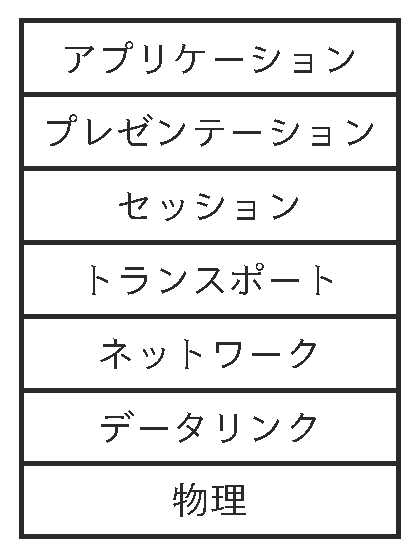
\includegraphics[width=5cm,pagebox=artbox]{figs/OSI.pdf}
    \caption{OSI参照モデル}
    \label{fig:osi}
\end{figure}

OSI自体は残らなかったが、OSI策定の際に考案されたOSI参照モデルと呼ばれる
ネットワークの抽象化手法は、今日でも広く受け入れられている。

\begin{itembox}[l]{\bf 重要ポイント}
    \begin{itemize}
        \item インターネット関連のプロトコルは、IETFが発行するRFCによって標準化されている
        \item コンピュータネットワークはレイヤで考えることができる
    \end{itemize}
\end{itembox}

\subsection{データリンク層}

\subsection{ネットワーク層}

\subsection{トランスポート層}

\subsection{トランスポートより上の層}